\documentclass[12pt]{article}

\usepackage[margin=1in]{geometry}
\usepackage{hyperref}
\usepackage{enumitem}
\usepackage{parskip}
\usepackage{booktabs}
\usepackage{array}
\usepackage{xcolor}
\usepackage{fancyhdr}
\usepackage{listings}
\usepackage{courier}
\usepackage{graphicx}
\usepackage{subcaption}

\definecolor{accent}{RGB}{50, 90, 160}
\definecolor{codegray}{RGB}{245,245,245}
\definecolor{codetxt}{RGB}{40,40,40}

% Header/footer
\pagestyle{fancy}
\fancyhf{}
\fancyhead[L]{\small\textit{Mini Game Hub}}
\fancyhead[R]{\small\textit{Project Report}}
\fancyfoot[C]{\thepage}
\renewcommand{\headrulewidth}{0.3pt}

% Code listing style
\lstset{
  backgroundcolor=\color{codegray},
  basicstyle=\footnotesize\ttfamily\color{codetxt},
  breaklines=true,
  frame=single,
  framerule=0.3pt,
  rulecolor=\color{gray},
  xleftmargin=6pt,
  xrightmargin=6pt,
  aboveskip=6pt,
  belowskip=6pt,
}

\hypersetup{
  colorlinks=true,
  linkcolor=accent,
  urlcolor=accent,
}

\title{CS108 Project Report: Mini Game Hub}
\author{
  \begin{tabular}{c @{\hspace{2.5cm}} c}
    Ritwik Khandelwal & Shreyas Lohiya \\
    25B1020           & 25B1094
  \end{tabular}
}
\date{CSE Department\\
Indian Institute Of Technology Bombay}


\begin{document}
\maketitle
\tableofcontents
\newpage

\section{Introduction}

Mini Game Hub is a two-player, turn-based game collection that runs on Linux. The project combines a Bash-based terminal front-end for authentication and navigation with a Python/Pygame graphical back-end for all gameplay. Two players log in (or sign up) through the terminal, choose a game and a visual theme, and then compete in a resizable Pygame window. Results are persisted to a CSV history file, which feeds a colourful leaderboard and a set of Matplotlib analytics plots.

The hub currently hosts four classic strategy games:
\begin{itemize}[noitemsep]
  \item \textbf{Tic-Tac-Toe} -- 10\(\times\)10 board, five-in-a-row variant.
  \item \textbf{Othello} -- Standard 8\(\times\)8 reversi rules.
  \item \textbf{Connect4} -- 7\(\times\)7-column drop-token game with physics animation.
  \item \textbf{Chain Reaction} -- Explosive chain-reaction strategy on a 9\(\times\)6 grid.
\end{itemize}

All games share a common object-oriented architecture through an abstract \texttt{Game} base class, ensuring consistency and ease of extension.

\section{External Libraries}

\begin{center}
\begin{tabular}{>{\bfseries}p{3.2cm} p{4cm} p{6.5cm}}
\toprule
Library & Version & Purpose \\
\midrule
pygame-ce & $\geq$ 2.5.7 & The primary framework for GUI rendering, event handling, and managing the game loop \\
numpy & $\geq$ 2.2.6 & Board representation, vectorised win-checking in games and animation math \\
matplotlib & $\geq$ 3.10.8 & In-game plots for top players across games, most played games by frequency, win distribution, PvP heat map \\
csv & stdlib & Reading \texttt{history.csv} inside the \texttt{plotstuff} method to aggregate win/loss/draw data without an external database. \\
datetime & stdlib & Stamping each game record with \texttt{date.today()} before appending to \texttt{history.csv}. \\
subprocess & stdlib & Launching \texttt{leaderboard.sh} from within Python, and removing the temporary \texttt{plot.png} after it has been loaded into Pygame. \\
sys & stdlib & Reading command-line arguments (\texttt{sys.argv}) to receive player usernames from the Bash launcher. \\
sha256sum & --- & Password encryption by converting plaintext into sha256 encoded string\\
column & --- & Terminal table formatting \\
\bottomrule
\end{tabular}
\end{center}

%% ─── 2. DESIGN & ARCHITECTURE ────────────────────────────────────────────────
\section{Design \& Architecture}

\textbf{Terminal UI} -- Interactive Terminal UI for signup and login with ASCII art and ANSI coloring

\textbf{Theme selection} -- Four background themes (Phonk, Futuristic, Retro, Space) selectable before each game session, including an option to select if you want the board to shake

\textbf{Animated game elements} --
  \begin{itemize}[noitemsep]
    \item Connect4: physics-accurate falling token (gravity + bounce damping).
    \item Tic-Tac-Toe / Connect4: animated win-line that draws itself progressively.
    \item Othello: ellipse-based coin-flip animation when pieces are outflanked.
    \item Chain Reaction: timed explosion animation with balls travelling to neighbours.
  \end{itemize}

\textbf{In-game controls} -- Resign button (forfeit immediately), Claim Draw button with Accept/Reject dialogue, and a Quit confirmation overlay.

\textbf{Animated UI elements} -- Menu title pulses sinusoidally; buttons scale up smoothly on hover with eased interpolation.

  

\subsection{Key Architectural Decisions}

\textbf{Inheritance-based game abstraction} All four games extend \texttt{game\_template}. The base class owns the main pygame loop, common UI elements (resign, claim draw, quit overlay), board panning via WASD, and board shaking. Each subclass only implements \texttt{win\_check}, \texttt{draw\_check}, \texttt{valid\_check}, \texttt{move}, \texttt{drawboard}, \texttt{specificmousepressevents}, and 2 or 3 helper functions for game logic and specific animations. This makes adding a new game straightforward and keeps the event loop DRY.

\textbf{Responsive layout} Every size — cell dimensions, font size, button positions — is derived from a single \texttt{smallerscalevalue} computed from the current window size relative to the reference resolution of $1280 \times 720$. A \texttt{VIDEORESIZE} event triggers \texttt{update()} which recomputes all layout values, making the application fully resizable.

\textbf{CSV history log} Game results are appended to \texttt{history.csv} in a simple five-field format: winner, loser, date, game name, is-draw flag. This flat file is parsed by both Python (for matplotlib plots) and awk (for the leaderboard), avoiding any database dependency.

\textbf{Single Game loop} This starts in the base class and calls the child classes and separate draw functions in the main loop. This maintains modularity of the code and truncates the loading time for repeated pygame initilizations.

\textbf{A button class} This class enables easy addition of buttons anywhere in the code which saves time for adding changes and new implementations.

%% ─── 3. FEATURES IMPLEMENTED ─────────────────────────────────────────────────
\section{Features Implemented}

\subsection{Authentication System (Bash)}
New users can sign up with a username (4–12 alphanumeric/underscore characters, must start with a letter) and a password (8–20 characters, must include upper, lower, digit, and one of \texttt{\_@\#\$\%\^{}\&*}). Passwords are stored as SHA-256 hashes in \texttt{users.tsv}. Login validates the hash. The second player cannot reuse the first player's username. A custom \texttt{readpass} function masks input with bullet characters.

\subsection{Main Menu \& Theme Selection}
After authentication the Python engine presents a game-selection menu followed by a theme-selection menu. Themes correspond to a background image and an audio track loaded at runtime, allowing new themes to be added very easily by dropping files into the \texttt{images/} and \texttt{audio/} directories and adding a string in line of code as

\texttt{theme=menu(self.screen,"CHOOSE A THEME","Phonk",}

\texttt{"Futuristic","Retro","Space","new-theme-name")}

\subsection{Resizable Pygame window} All board positions, cell sizes, fonts, and button geometry scale with the window to make it look playable and resize the side according to your preference at the same time.

\subsection{Chain Reaction}
Chain-Reaction is implemented in addition to the three specified games, it is a cult classic phone game which has an interesting recursive logic and a decent animation implementation.

\subsection{In-Game Controls}
All games share resign buttons (immediately awards win to the opponent), claim-draw buttons (opponent must accept or reject), a quit-confirmation overlay, and WASD / arrow-key board panning.

\subsection{Leaderboard}
Accessible both from the shell (before launching Python) and from the post-game menu. Metrics: Username, Wins, Win\%, Losses, Loss\%, Wins/Losses. Data is broken down per game and combined. The terminal table is rendered with box-drawing characters and ANSI colour codes using awk.

\subsection{Statistics Plots}
Four matplotlib views: Top 5 Players (bar chart), Total Wins (pie), Most Played Games (pie), and a PvP heat map showing the net win differential between every pair of players. Plots are saved to a temporary PNG and displayed inside the pygame window.

\subsection{Animation as time-based interpolation} Animations (falling tokens in Connect4, flipping discs in Othello, exploding orbs in Chain Reaction, win-line drawing in Tic-Tac-Toe / Connect4) are driven by elapsed wall-clock time rather than frame counters, so they behave consistently regardless of frame rate.
\newpage
%% ─── 4. DIRECTORY STRUCTURE ──────────────────────────────────────────────────
\section{Directory Structure}

\begin{lstlisting}
mini-game-hub/
|-- main.sh              # Shell entry point
|-- leaderboard.sh       # Terminal leaderboard renderer
|-- game.py              # Python entry point: GameEngine, stat plots
|-- history.csv          # Append-only game result log
|-- users.tsv            # Username and SHA-256 password hash store
|-- games/
|   |-- game_template.py # Abstract base class; owns the main pygame loop
|   |-- tictactoe.py     # 10x10 five-in-a-row Tic-Tac-Toe
|   |-- othello.py       # 8x8 Othello 
|   |-- connect4.py      # 7x7 Connect4 with physics drop animation
|   `-- chainreaction.py # 9x6 Chain Reaction with cascade explosions
|-- ui/
|   |-- button.py        # Hover-animated Button widget
|   |-- menu.py          # Reusable option-menu screen
|   |-- welcome.py       # Welcome splash screen
|   `-- thankyou.py      # Exit / thank-you screen
|-- images/              # Background PNGs per theme; X/O/board token images; jpegs for report
|-- audio/               # .ogg background music tracks (one per theme)
|-- fonts/               # BlackgothRegular.otf display font
|-- Makefile             # Makefile for pdflatex
|-- report.tex           # Latex report code
`-- report.pdf           # Latex report pdf

\end{lstlisting}

%% ─── 5. INSTALLATION & SETUP ─────────────────────────────────────────────────
\section{Installation \& Setup}

\textbf{Requirements:} Python 3.10+, Bash, standard POSIX utilities (\texttt{awk}, \texttt{sort}, \texttt{column}, \texttt{sha256sum}).\\
If column is not installed do:

\texttt{sudo apt install column}

Install python dependencies from requirements.txt:

\texttt{pip install -r requirements.txt}

\begin{lstlisting}
pygame-ce==2.5.7
numpy==2.2.6
matplotlib==3.10.8
\end{lstlisting}

Make shell scripts executable and run:

\begin{lstlisting}[language=bash]
chmod +x main.sh leaderboard.sh
./main.sh
\end{lstlisting}

\textbf{Assets:} The \texttt{images/}, \texttt{audio/}, and \texttt{fonts/} directories must be present alongside the scripts.
\newpage
%% ─── 6. USAGE ────────────────────────────────────────────────────────────────
\section{Usage}

Run \texttt{./main.sh} from the project root in a terminal. The shell script walks through the following flow:

\begin{figure}[h]
    \centering

    \begin{subfigure}{0.45\textwidth}
        \centering
        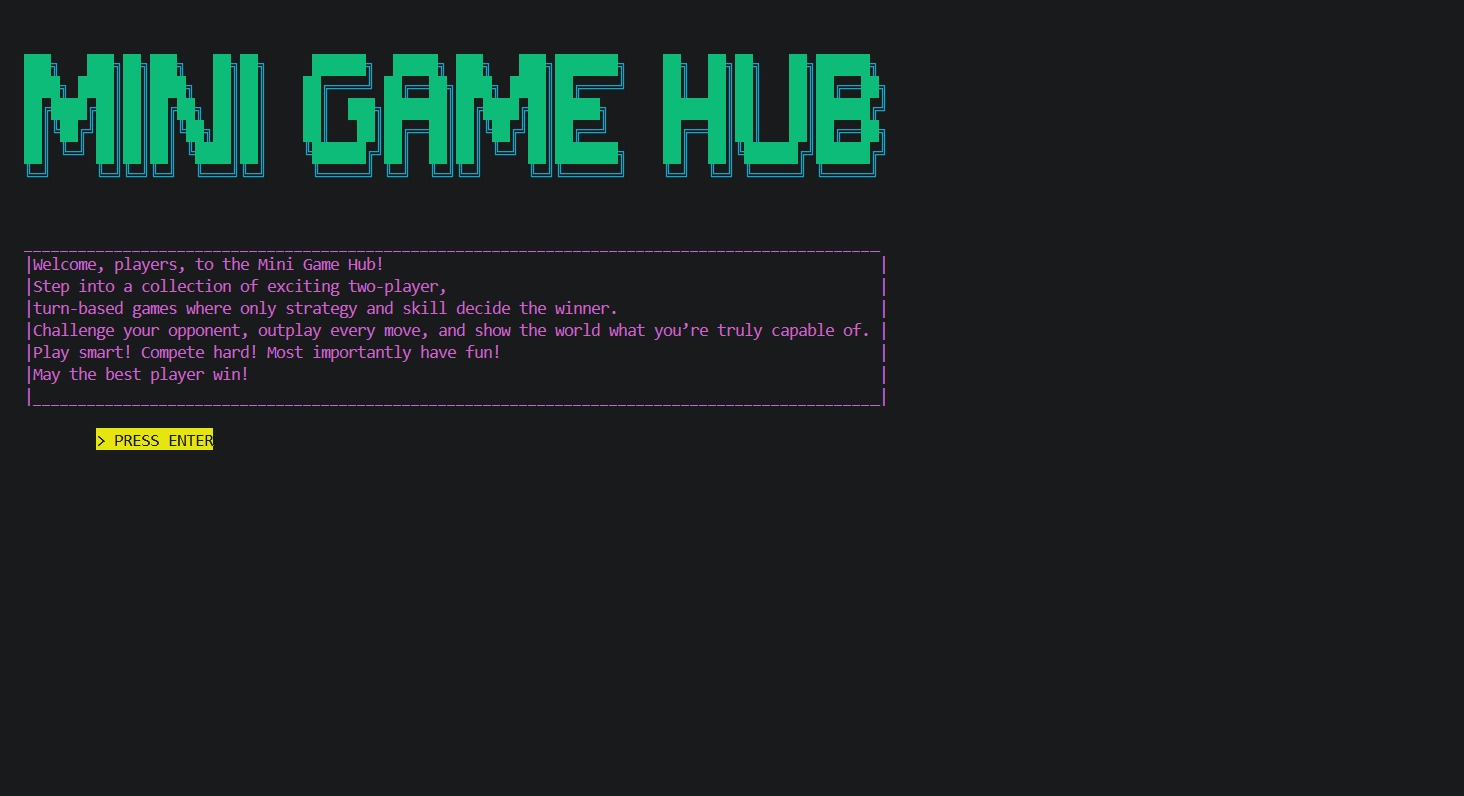
\includegraphics[width=\linewidth]{images/image1.jpeg}
        \caption{Welcome screen — press Enter to continue.}
    \end{subfigure}
    \hfill
    \begin{subfigure}{0.45\textwidth}
        \centering
        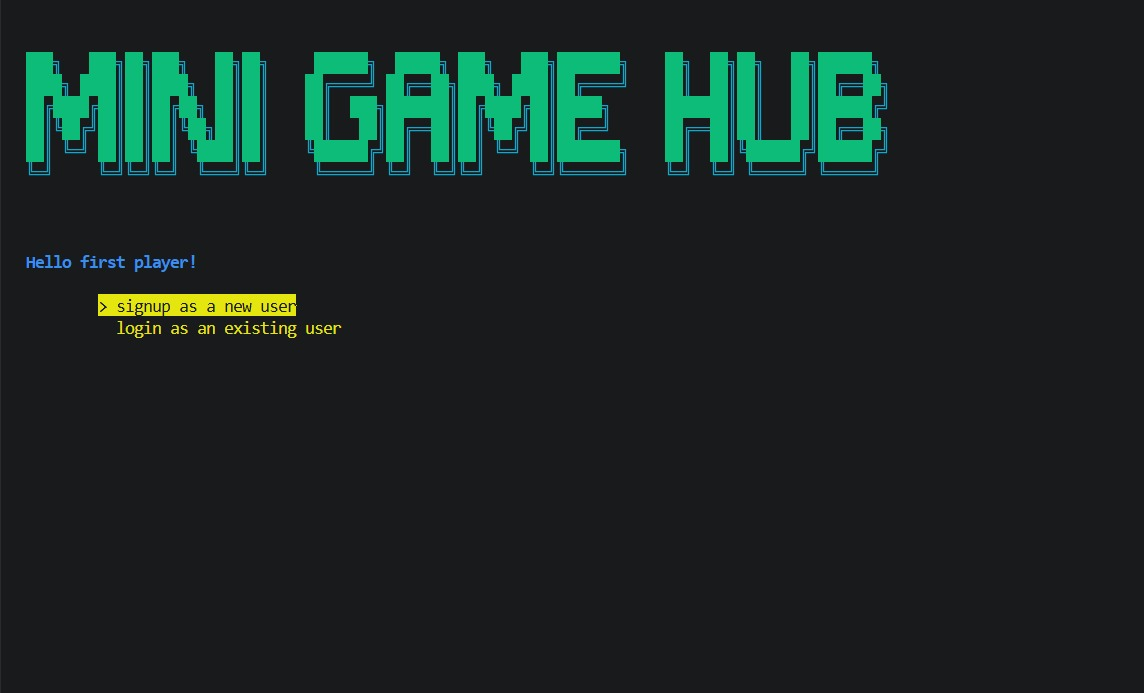
\includegraphics[width=\linewidth]{images/image2.jpeg}
        \caption{Play or Leaderboard — view leaderboard or proceed to play}
    \end{subfigure}

    \vspace{0.5cm}

    \begin{subfigure}{0.45\textwidth}
        \centering
        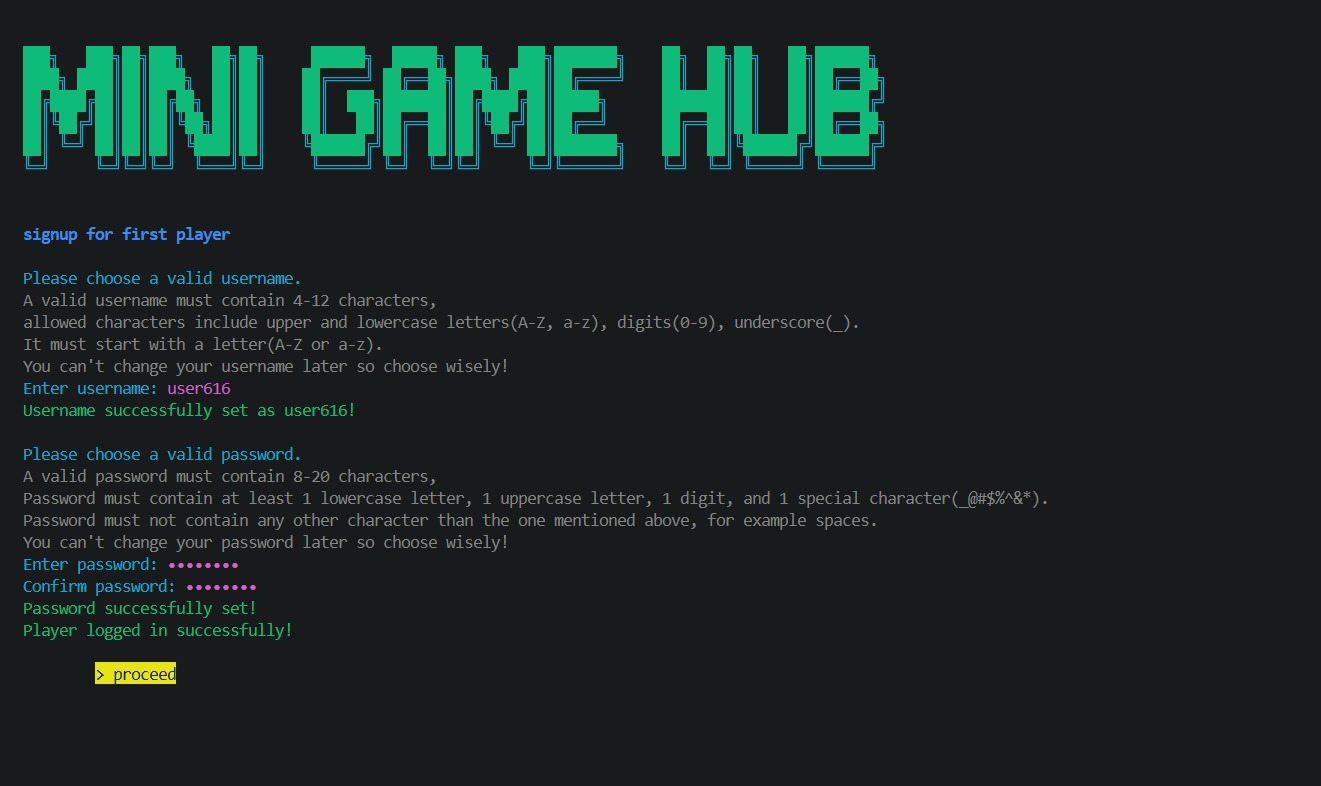
\includegraphics[width=\linewidth]{images/image3.jpeg}
        \caption{Authentication — players sign up}
    \end{subfigure}
    \hfill
    \begin{subfigure}{0.45\textwidth}
        \centering
        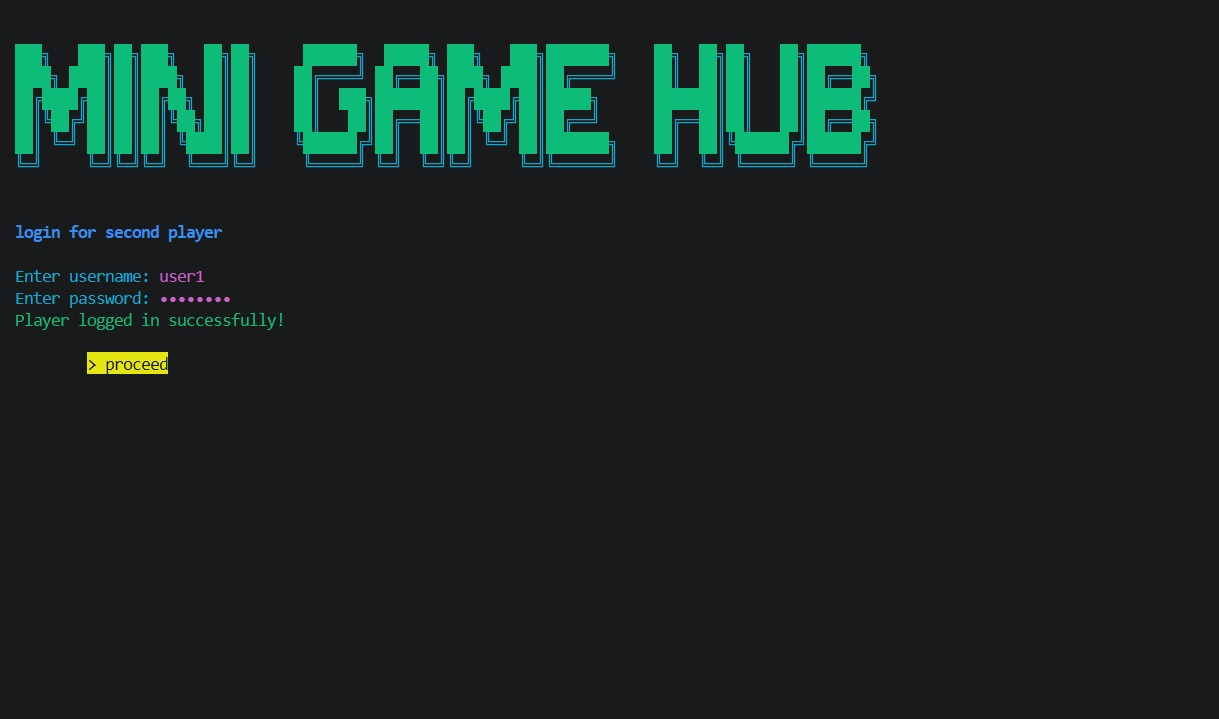
\includegraphics[width=\linewidth]{images/image4.jpeg}
        \caption{Players log in}
    \end{subfigure}

    \caption{Application flow screens}
\end{figure}

\begin{enumerate}[leftmargin=*, itemsep=2pt, start=2]
  \item \textbf{Game selection} — choose Tic-Tac-Toe, Othello, Connect4, or Chain Reaction.
  \item \textbf{Theme selection} — choose Phonk, Futuristic, Retro, or Space.
  \item \textbf{Gameplay} — click cells to place pieces. Use WASD / arrow keys to pan the board. Resign or claim draw via the side buttons. Press Escape for the quit overlay.
  \item \textbf{Post-game} — view the leaderboard, view plots, play again, or quit.
\end{enumerate}

\textbf{Keyboard shortcuts:} W/A/S/D or arrow keys pan the board. Escape opens the quit-confirmation overlay.

%% ─── 7. RETROSPECTIVE ────────────────────────────────────────────────────────
\section{Retrospective}

\subsection{Challenges}

\textbf{Resizable Window Scaling} -- The most tedious challenge was making every UI element board cells scale correctly when the user resizes the Pygame window. A single \texttt{smallerscalevalue} factor was adopted, and all pixel measurements were multiplied by it one by one which was a tedious task. The \texttt{update()} method on \texttt{Game} reconstructs every button and reloads the font at the new size upon each \texttt{VIDEORESIZE} event.


\textbf{Othello Turn Skipping and Game End} -- Standard Othello requires passing a turn when a player has no legal moves, and ending the game when \emph{both} players are locked. The overridden \texttt{switch\_turn()} method handles this by probing all cells for valid moves after each switch, and calling \texttt{win\_check()} only when neither player can act.

\textbf{Modular Implementation of Animation} -- Implementing Animation as a loop in a separate function outside the game loop proved to be useless as it stopped running the original loop and freezed the board. Adding the code directly in the game loop was also ugly and depreived the code of its modularity. So a function made for drawing each frame separately in the loop on the basis of when the bool value which changed on need to do basis and worked smoothly.

\textbf{Single Game Loop} -- Required effective directory management and proper function and class definitions across co-classes and child-classes

\textbf{Physics animation in Connect4} -- Simulating realistic bouncing without a physics engine required deriving closed-form expressions for the position of the token at each frame using kinematics equations, a coefficient of restitution, and a bounce-count cap to prevent infinite micro-bounces.

\textbf{Team-Work}

\subsection{What We Would Do Differently}

\begin{enumerate}[leftmargin=*, label=\textbf{\arabic*.}]

\item \textbf{Replay system.} Record every move to the history file and build a replay viewer that steps through past games frame-by-frame, which would be especially compelling for Chain Reaction chains.

\item \textbf{Undo/take-back mechanic.} Maintain a move stack per game and allow both players to agree to undo the last move -- useful for casual play. Also the move stack could be used for reviewing game like in chess for analysis later.

\end{enumerate}
\newpage
%% ─── 8. REFERENCES ───────────────────────────────────────────────────────────
\section{References}

\begin{enumerate}[leftmargin=*, itemsep=2pt]
  \item Pygame documentation — \url{https://www.pygame.org/docs/ }, 
  \url{https://pyga.me/}
  \item NumPy documentation — \url{https://numpy.org/doc/} and Bodhitree
  \item Matplotlib documentation — \url{https://matplotlib.org/stable/} and Bodhitree
  \item \textit{Chain Reaction} game rules — \url{https://en.wikipedia.org/wiki/Chain_Reaction_(game)}
  \item \textit{Reversi / Othello} game rules — \url{https://en.wikipedia.org/wiki/Reversi}
  \item ANSI escape codes reference — \url{https://en.wikipedia.org/wiki/ANSI_escape_code}
  \item GNU awk manual — \url{https://www.gnu.org/software/gawk/manual/} and Bodhitree
  \item Background Images - AI Generated
\end{enumerate}

\end{document}